% NIME 2020 Music Proceedings Template

% Modified November 2024 by Charles Martin
% Modified December 2019 by Joe Wright
% Created August 2019 by Niccolo Granieri
% This is file `music-proceedings-template.tex',

\documentclass{nimemusic}


\usepackage{lipsum} %used to generate default text
% Rights management information.
\setcopyright{cc4}
\nimeYear{2024}
\nimeMonth{9}
% \nimeDOI{10.1145/XXXXXXX.XXXXXXX}
% \whichProceedings{Music Proceedings of the International Conference on New Interfaces for Musical Expression}
\whichNIME{NIME'25, June 24--27, 2025. The Australian National University, Canberra, Australia.}

\begin{document}

\title{Title: Your NIME Music Performance}



% The "author" command and its associated commands are used to define
% the authors and their affiliations.
% Of note is the shared affiliation of the first two authors, and the
% "authornote" and "authornotemark" commands
% used to denote shared contribution to the research.
\author{Author One}
\affiliation{%
  \institution{Affilitation \#1}
  \city{City}
  \country{Country}
}

\author{Author Two}
\affiliation{%
  \institution{Affilitation \#1}
  \city{City}
  \country{Country}
}

\author{Author Three}
\affiliation{%
  \institution{Affilitation \#1}
  \city{City}
  \country{Country}
}


% By default, the full list of authors will be used in the page
% headers. Often, this list is too long, and will overlap
% other information printed in the page headers. This command allows
% the author to define a more concise list
% of authors' names for this purpose.
% \renewcommand{\shortauthors}{One, Two and Three}


% Keywords. The author(s) should pick words that accurately describe
% the work being presented. Separate the keywords with commas.
\keywords{datasets, neural networks, gaze detection, text tagging}


% This command processes the author and affiliation and title
% information and builds the first part of the formatted document.
\maketitle


\section{Program Notes}

\lipsum[1] 

Plus, some citations to articles: \cite{doe2023,
wizard2022, alien2024}.

\begin{figure}[hbt]
  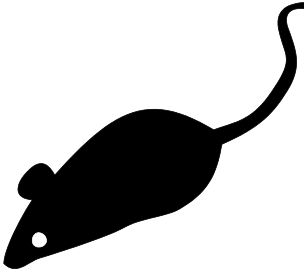
\includegraphics{NIME_Mouse}
  \caption{The NIME Mouse}
\end{figure}


\section{Project Description}

\lipsum[2]

\section{Technical Notes}

\lipsum[3]

\section{Media Links}

\begin{itemize}
	\item Video: \url{www.yournimevideolink.com/younameit}
	\item Audio: \url{www.yournimeaudiolink.com/younameit}
\end{itemize}


% The acknowledgements section is optional and can be removed if not needed.
\begin{acks}
The authors would like to thank\ldots
\\
This work was supported by\ldots
\end{acks}

\section*{Ethical Standards}

Please note that an Ethical Standards section is required for NIME submissions.

This could include information regarding sources of funding, sustainability factors, potential conflicts of interest,  informed consent if the research involved human participants, statement on welfare of animals if the research involved animals, or other ethical factors that are relevant to the work.

% bibliography style
\bibliographystyle{ACM-Reference-Format}
% reference file
\bibliography{references}
\end{document}
